
\item One mole of a monatomic ideal gas undergoes four thermodynamic processes as shown schematically in the PV-diagram below. Among these four processes, one is isobaric, one is isochoric, one is isothermal and one is adiabatic. Match the processes mentioned in List-1 with the corresponding statements in List-II.

    \begin{center}
        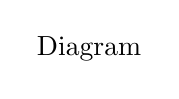
\begin{tikzpicture}
            \node {Diagram};
        \end{tikzpicture}
    \end{center}

    \begin{center}
        \renewcommand{\arraystretch}{2}
        \begin{table}[h]
            \centering
            \begin{tabular}{p{0.25cm}p{4cm}|p{0.25cm}p{9cm}}
            \hline
            & List-I & & List-II \\
            \hline
            P & In process I & 1 & Work done by the gas is zero \\
            Q & In process II & 2 & Temperature of the gas remains unchanged \\
            R & In process III & 3 & No heat is exchanged between the gas and its surroundings \\
            S & In process IV & 4 & Work done by the gas is \(6P_0V_0\) \\
            \hline
            \end{tabular}
        \end{table}
    \end{center}

    \begin{tasks}(2)
        \task \( P \to 4 \), \( Q \to 3 \), \( R \to 1 \), \( S \to 2 \)
        \task \( P \to 1 \), \( Q \to 3 \), \( R \to 2 \), \( S \to 4 \)
        \task \( P \to 3 \), \( Q \to 4 \), \( R \to 1 \), \( S \to 2 \)
        \task \( P \to 3 \), \( Q \to 4 \); \( R \to 2 \), \( S \to 1 \)
    \end{tasks}